%% Resluts chapter
%% author Liu Peng

After designing, implementing and testing the software. We started several
evaluation tests on the streaming performance, and we have released the
application to public in Nov 2013. So far, we have improved the application a
lot and also brought many new features to it. As discussed in previous chapter,
we used Google Analytics SDK to help us get insights to our application and our
users. In this chapter we will present and analyze those results.

\subsection{Performance}
In terms of streaming, our solution include two major streaming components. It
would be helpful to study how the media streaming protocol have the better 
performance while streaming multimedia contents. And also, by comparing
different streaming types of media, we could investigate which protocol is best
suitable for certain type of media. Two major streaming technology we
used in our solution are HTTP streaming and RTSP streaming.

Hypertext Transfer Protocol (HTTP) refers to the protocol used to deliver web
pages and images across the Internet worldwide. HTTP is an adopted, open
standard-the most ubiquitous mode of delivery on-line. HTTP is a "stateless"
protocol; think of it as an airline ticket to anywhere. HTTP can be delivered
by a variety of web servers, both commercial and open source.

Real Time Streaming Protocol (RTSP) is a network control protocol used in
entertainment and communications systems to control streaming media servers.
RTSP is used to establish and control media sessions between two points,
usually server and player client. Clients of media servers issue VCR-like
commands, such as PLAY and PAUSE, to facilitate real-time control of playback
of media files from the server. Microsoft's Smooth Streaming is a hybrid
delivery method that acts like traditional RTSP streaming but is based on HTTP
PDL. Apple's HTTP Live Streaming (HLS) is another example of using HTTP to
deliver video with new techniques.

AirPlay uses RTSP streaming for the iTunes music. Thus we chose a mp3 music and
try to stream it to an AirPlay Speaker and an DLNA Speaker, and we used
Wireshark running on rooted Android phone to capture the packets in the network.
The result is presented below, the initial packet count is relatively high,
this is because there is a lot multicast messages in the network for device
discovery, after that, streaming graph shows that after an initial increase in
the traffic, network traffic is relatively stable, this is because the TCP
protocol reaches the best optimized transmission speed.

Next step, we added packet loss in the network, and see the influence to the two
streaming process, result is shown below:
\begin{figure}[H]
\begin{minipage}[b]{0.45\linewidth}
\centering
\includegraphics[width=\textwidth]{charts/AirPlay_traffic_data}
%%\hspace{0.1cm}
\end{minipage}
\begin{minipage}[b]{0.45\linewidth}
\centering
\includegraphics[width=\textwidth]{charts/AirPlay_traffic_5loss_data}
\end{minipage}
\begin{minipage}[b]{0.45\linewidth}
\centering
\includegraphics[width=\textwidth]{charts/AirPlay_traffic_10loss_data}
%%\hspace{0.1cm}
\end{minipage}
\begin{minipage}[b]{0.45\linewidth}
\centering
\includegraphics[width=\textwidth]{charts/AirPlay_traffic_15loss_data}
\end{minipage}
\caption{AirPlay streaming performance in terms of packet loss}\label{multiavp}
\end{figure}



\begin{figure}[H]
\begin{minipage}[b]{0.45\linewidth}
\centering
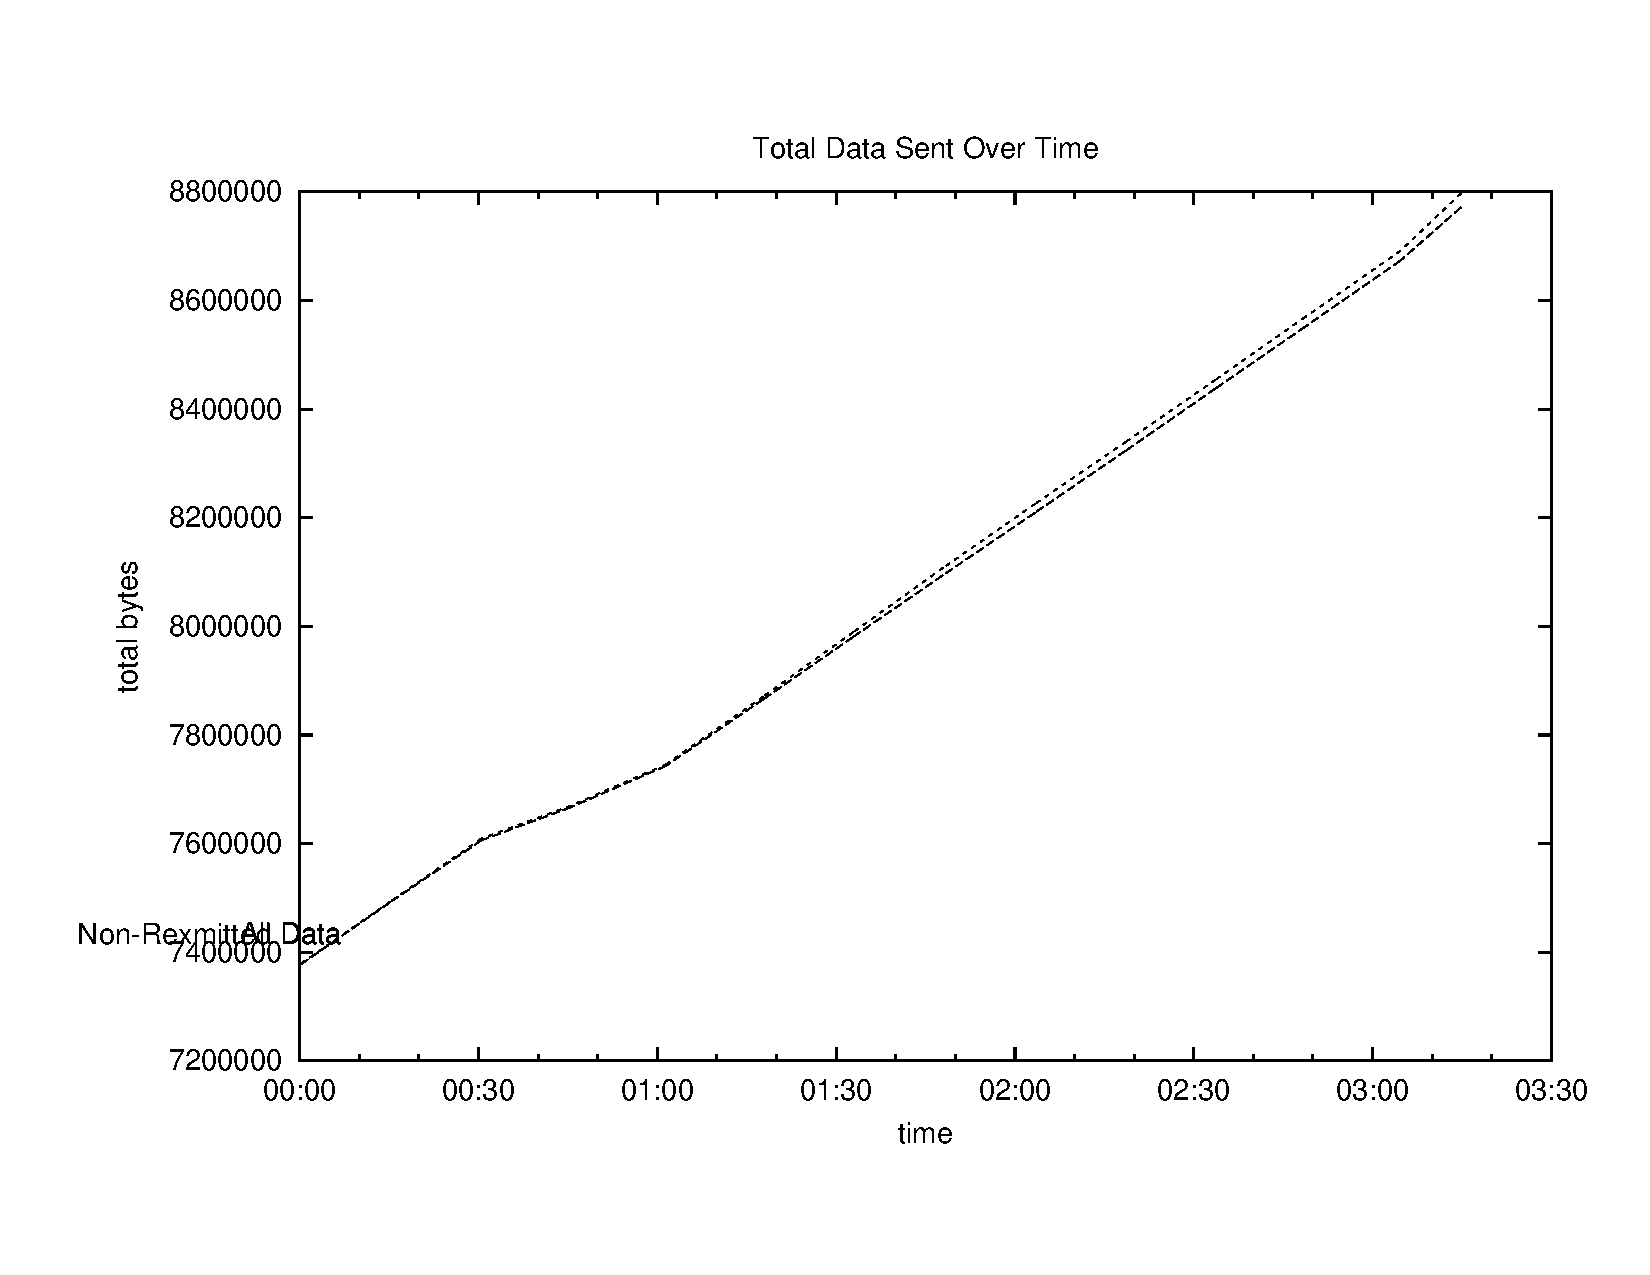
\includegraphics[width=\textwidth]{charts/dlna_traffic_data}
%%\hspace{0.1cm}
\end{minipage}
\begin{minipage}[b]{0.45\linewidth}
\centering
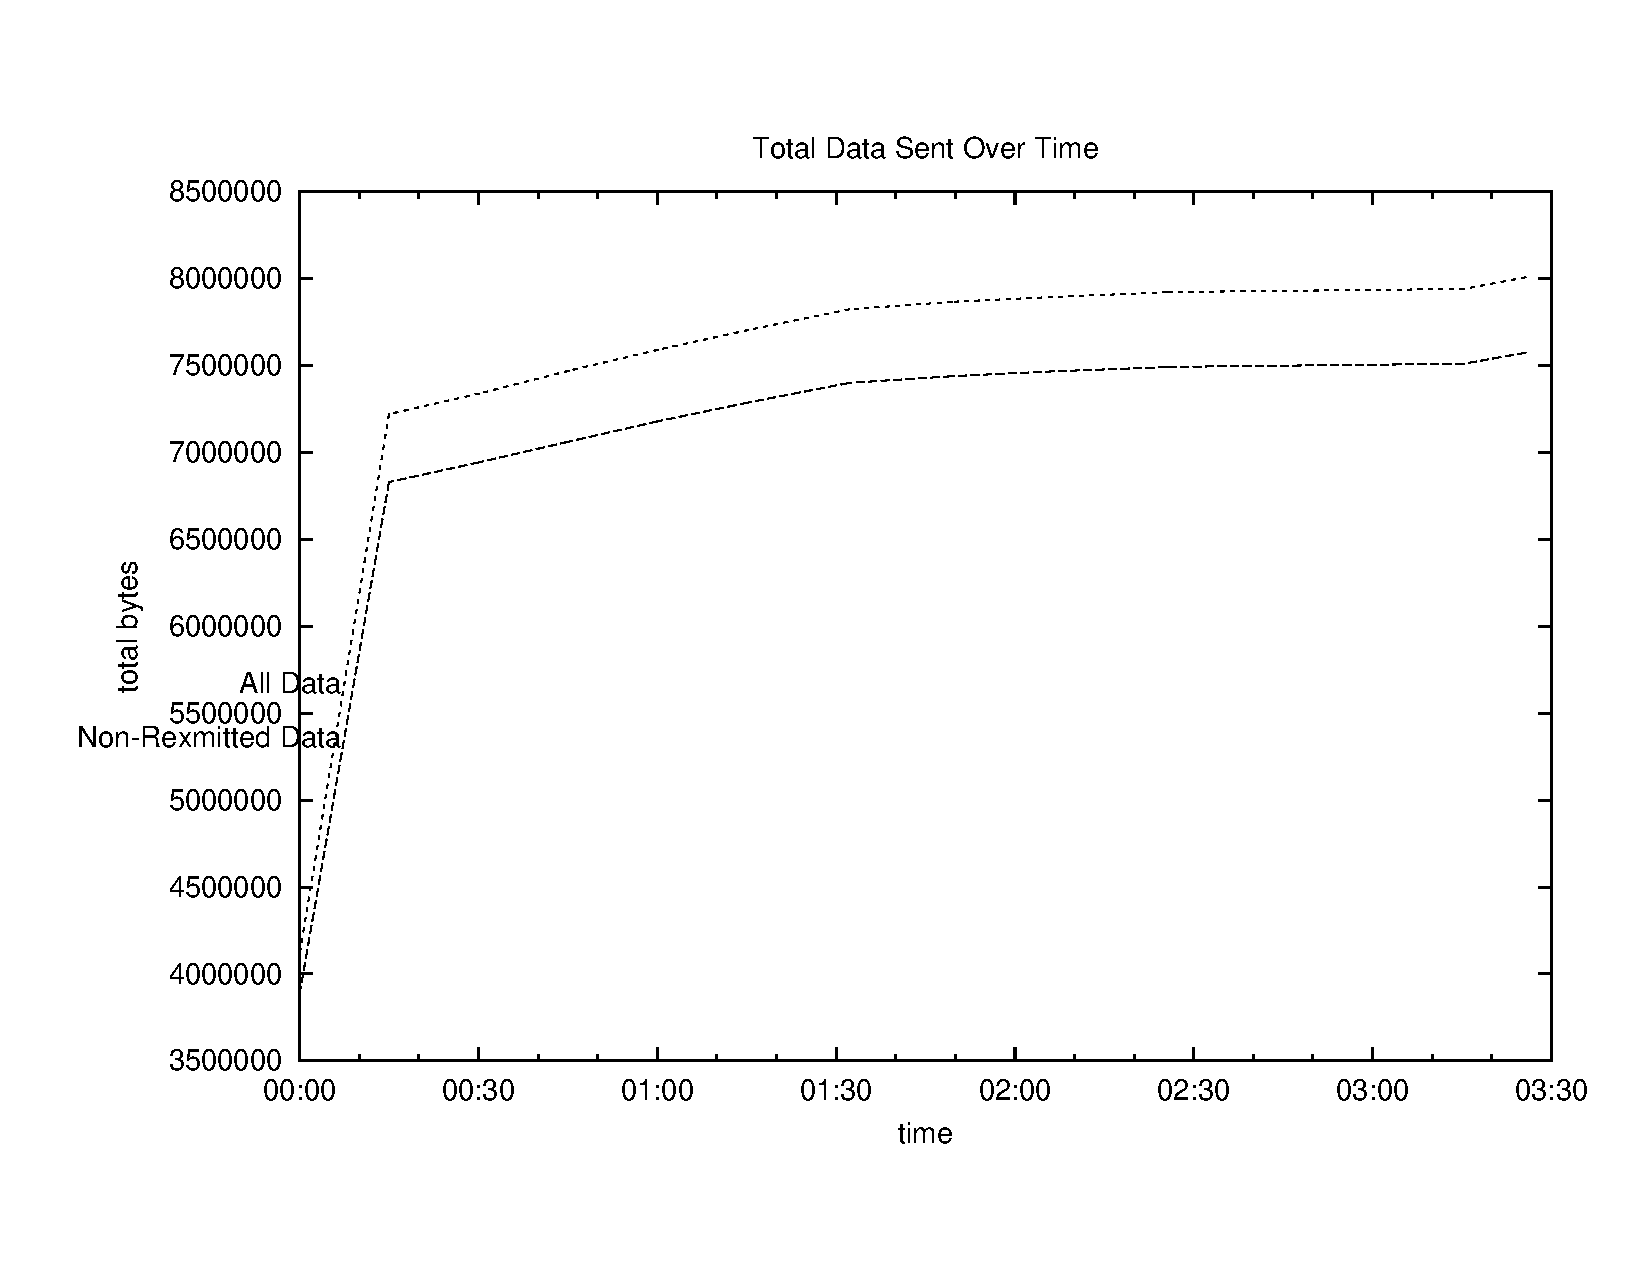
\includegraphics[width=\textwidth]{charts/dlna_traffic_5loss_data}
\end{minipage}
\begin{minipage}[b]{0.45\linewidth}
\centering
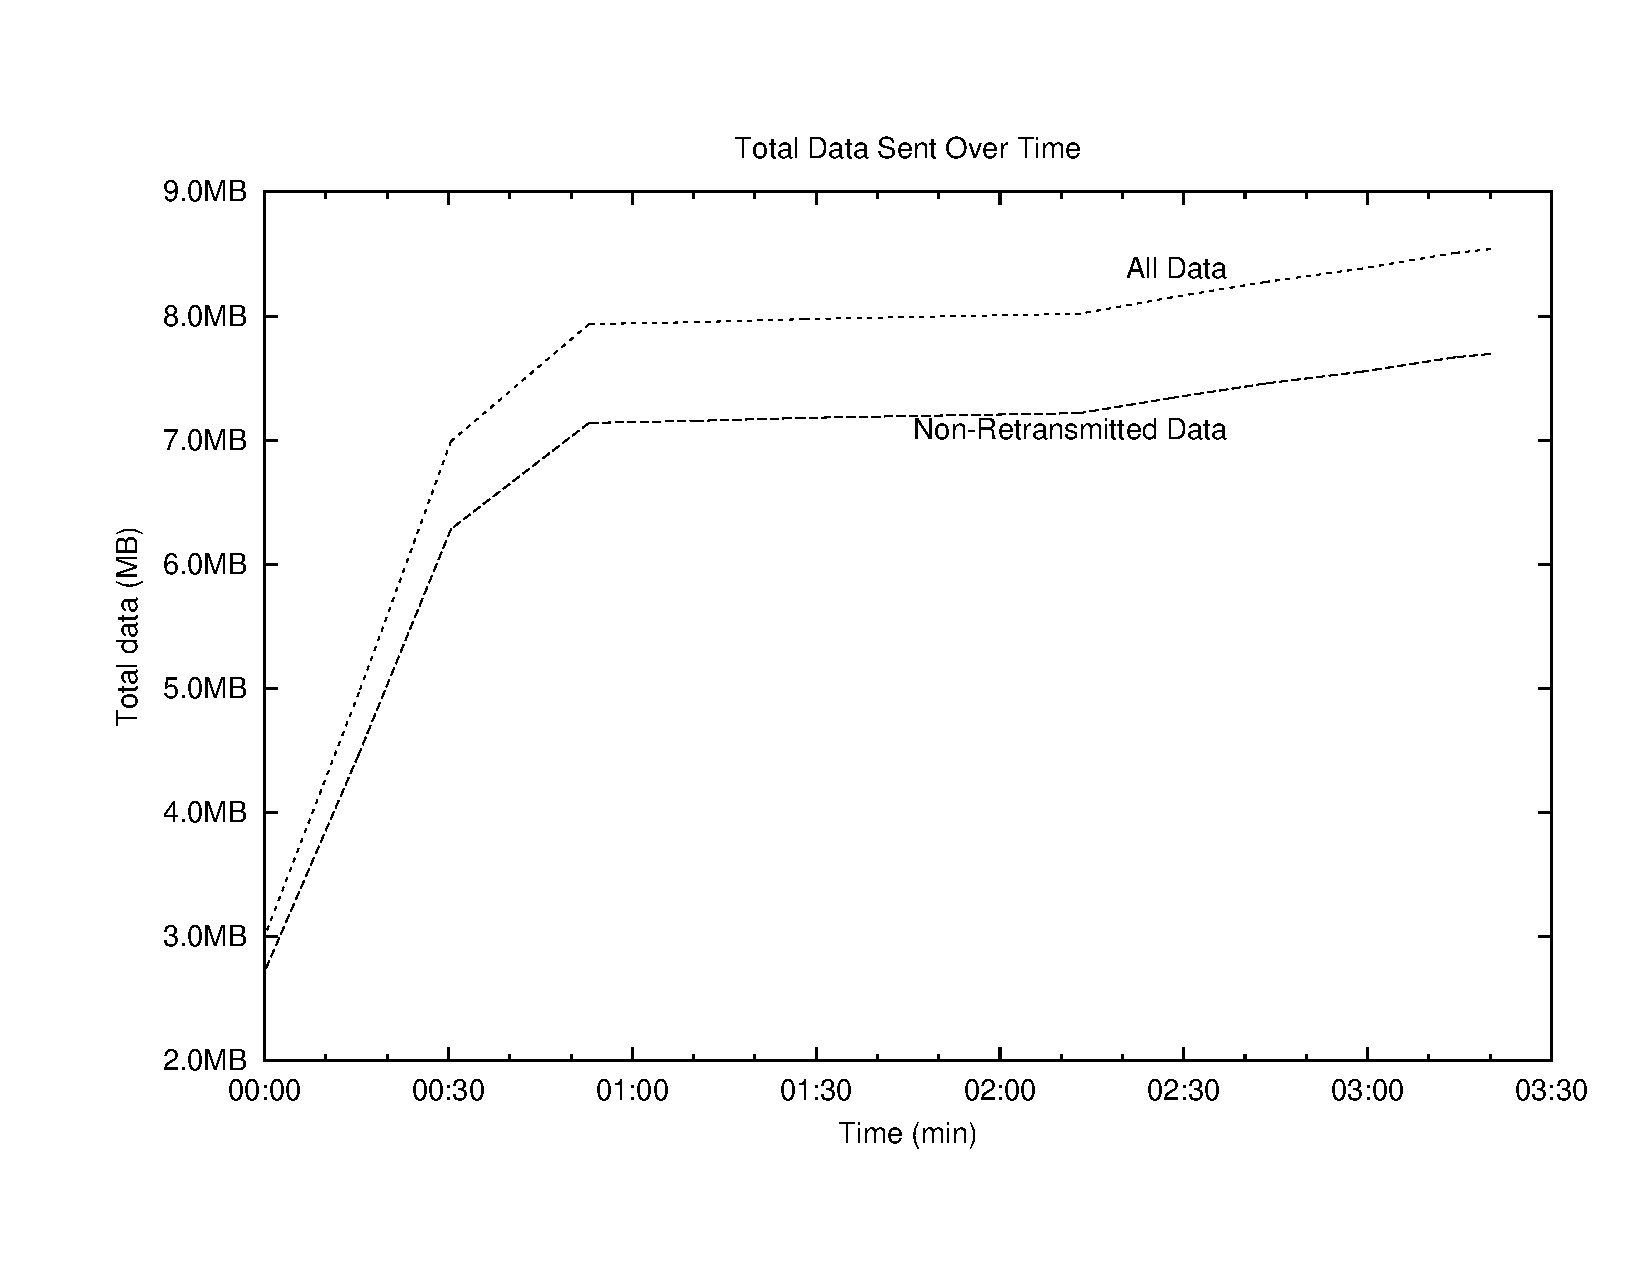
\includegraphics[width=\textwidth]{charts/dlna_traffic_10loss_data}
%%\hspace{0.1cm}
\end{minipage}
\begin{minipage}[b]{0.45\linewidth}
\centering
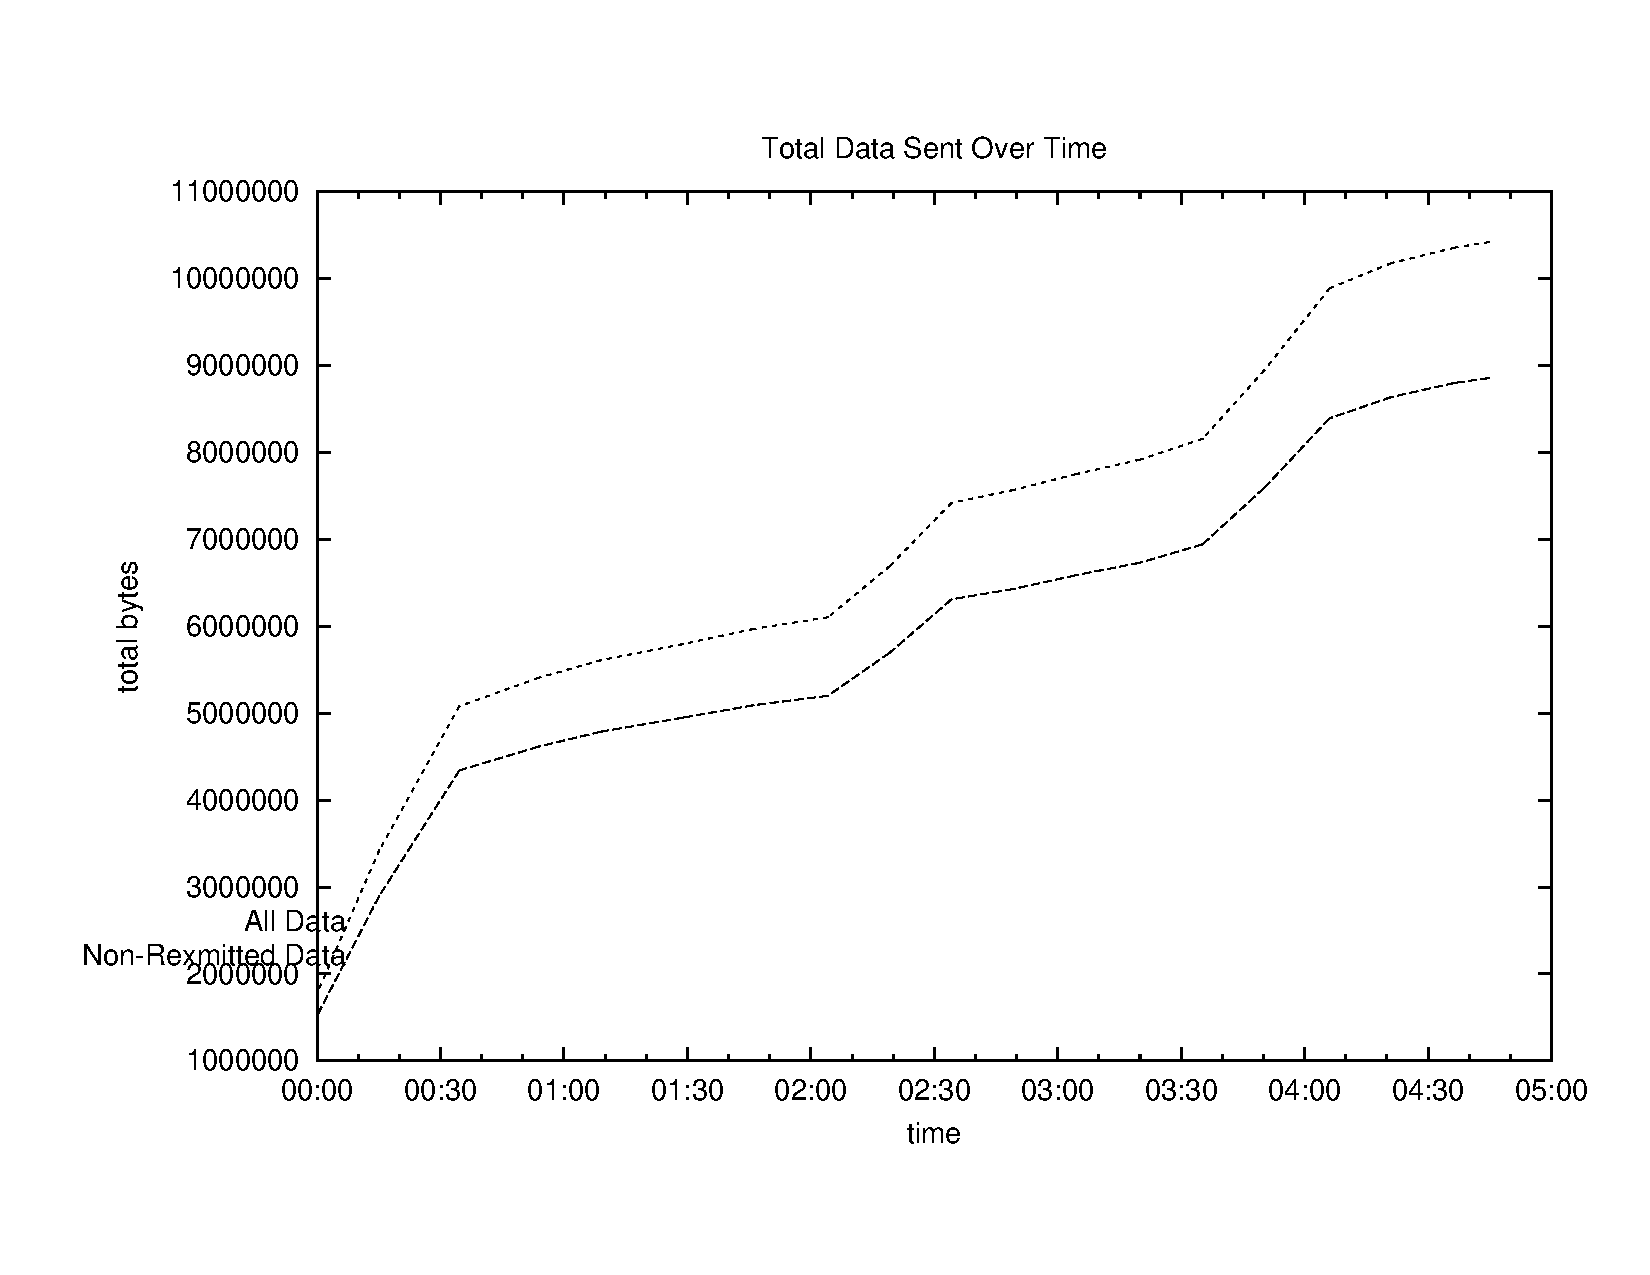
\includegraphics[width=\textwidth]{charts/dlna_traffic_15loss_data}
\end{minipage}
\caption{DLNA streaming performance in terms of packet loss}\label{multiavp}
\end{figure}

\begin{figure}[htb]
\centering \includegraphics[height=10cm]{charts/AirPlay_traffic_data}
\caption{AirPlay traffic data chart \label{chart6}}
\end{figure}
\begin{figure}[htb]
\centering 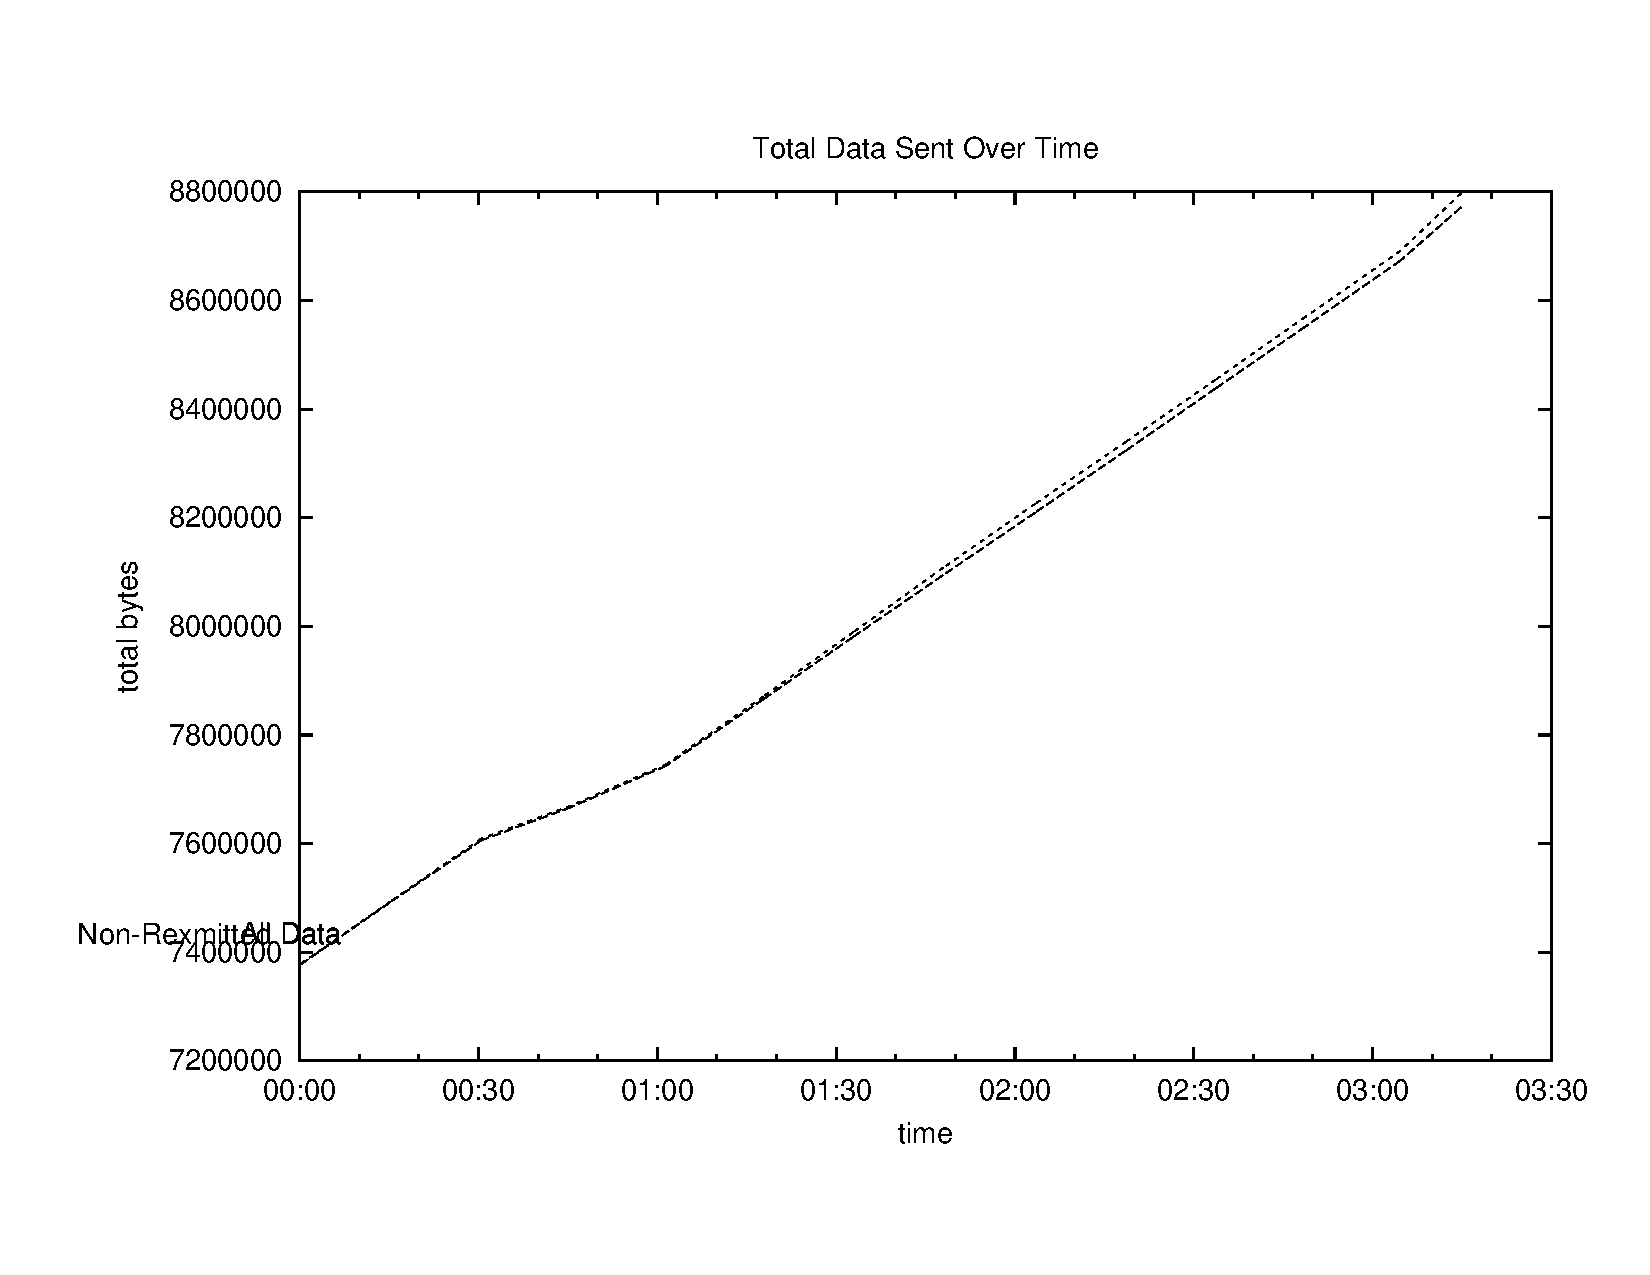
\includegraphics[height=10cm]{charts/dlna_traffic_data}
\caption{DLNA traffic data chart \label{chart6}}
\end{figure}

\begin{figure}[htb]
\centering \includegraphics[height=10cm]{charts/badnetwork_AirPlay_traffic_data}
\caption{AirPlay bad network traffic data chart \label{chart6}}
\end{figure}
\begin{figure}[htb]
\centering 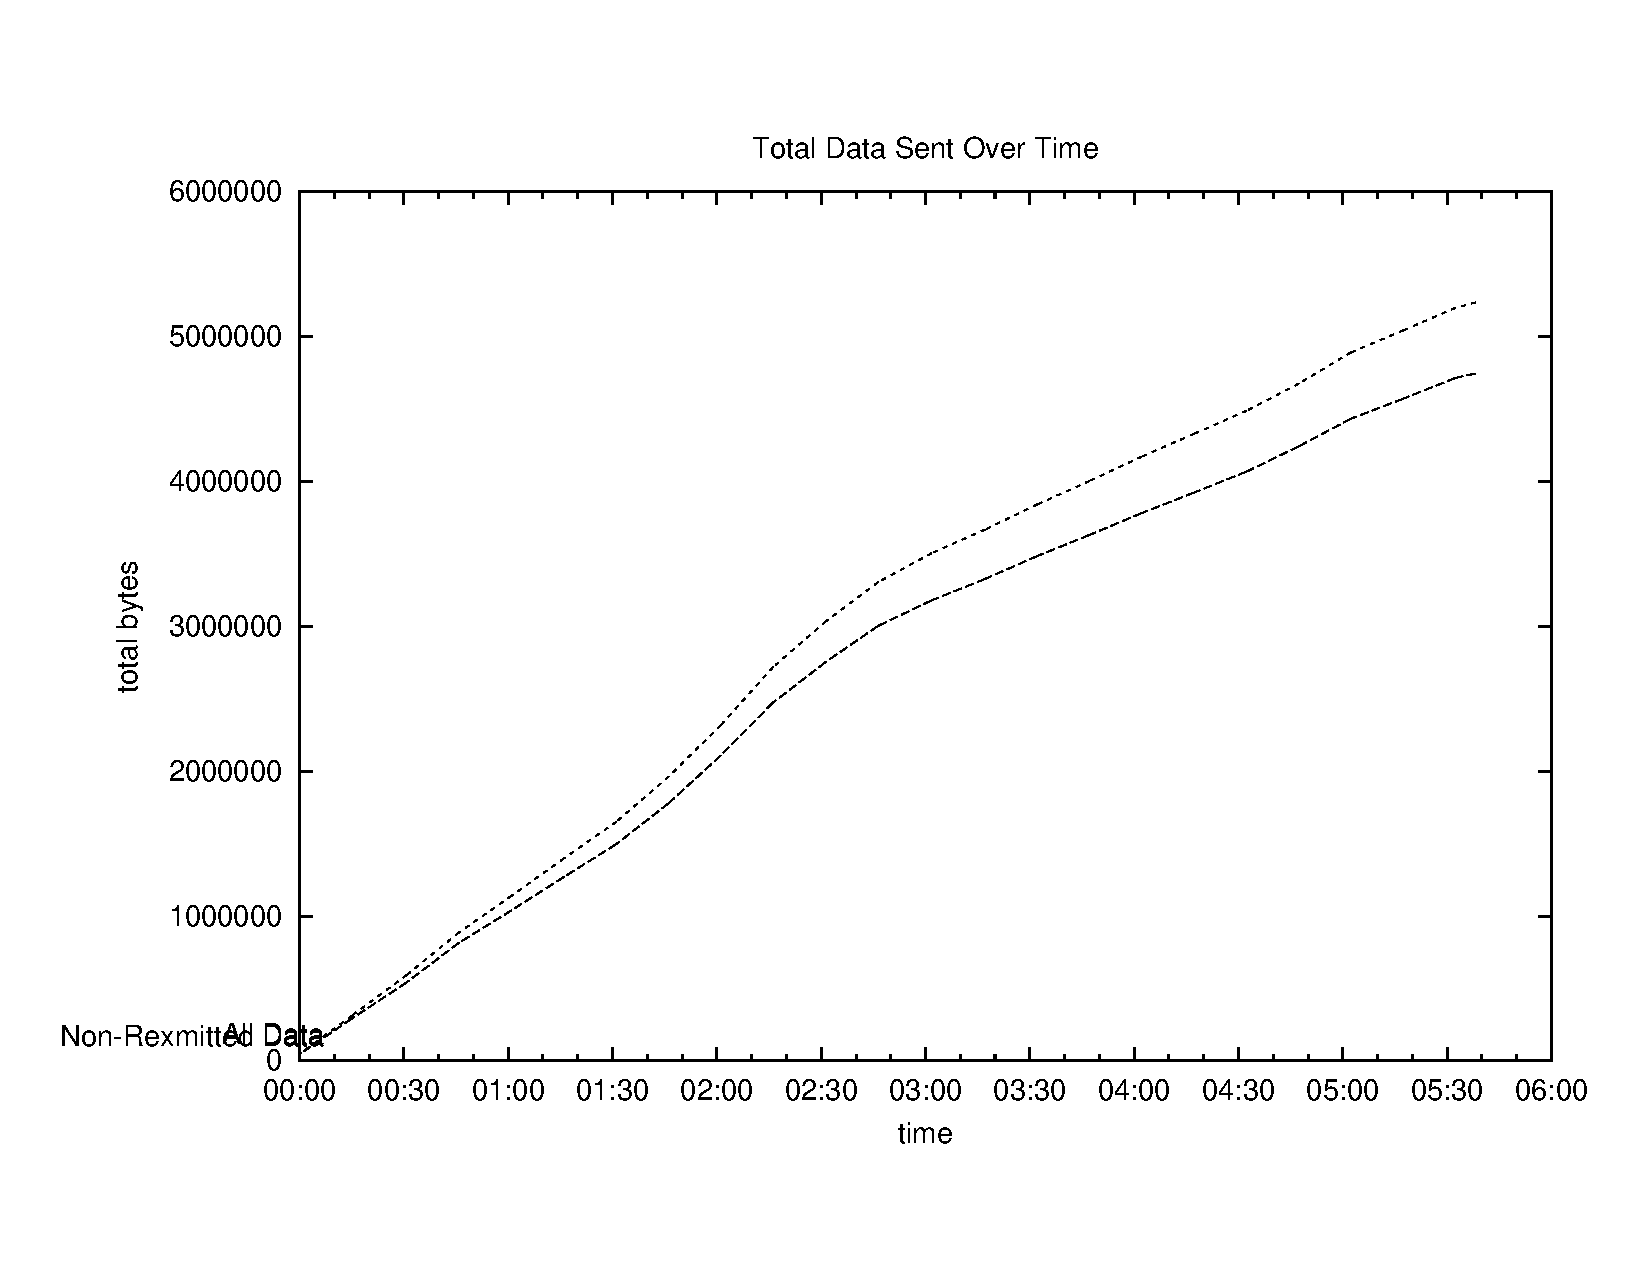
\includegraphics[height=10cm]{charts/badnetwork_dlna_traffic_data}
\caption{DLNA bad network traffic data chart \label{chart6}}
\end{figure}


\begin{figure}[htb]
\centering \includegraphics[height=10cm]{charts/AirPlay_traffic_5loss_data}
\caption{AirPlay bad network traffic data chart \label{chart6}}
\end{figure}
\begin{figure}[htb]
\centering 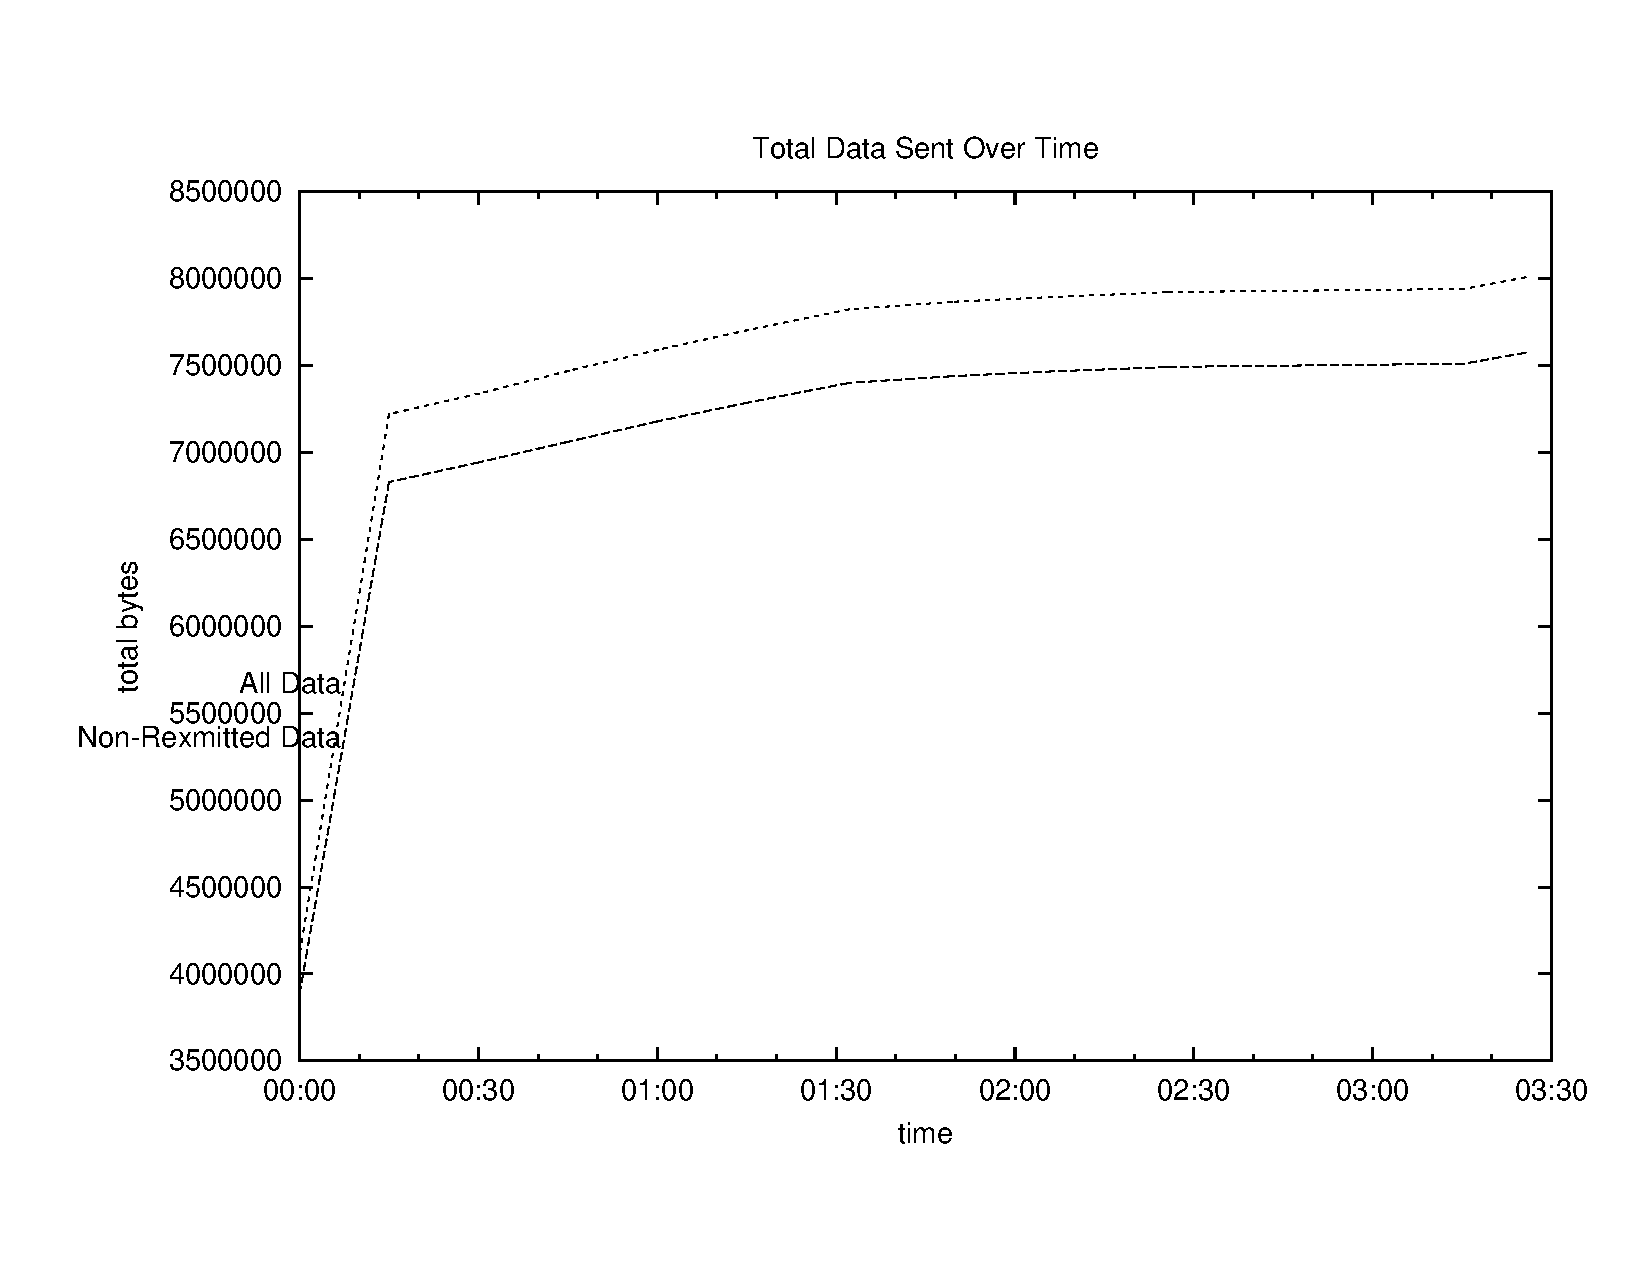
\includegraphics[height=10cm]{charts/dlna_traffic_5loss_data}
\caption{DLNA bad network traffic data chart \label{chart6}}
\end{figure}


\begin{figure}[htb]
\centering \includegraphics[height=10cm]{charts/AirPlay_traffic_10loss_data}
\caption{AirPlay bad network traffic data chart \label{chart6}}
\end{figure}
\begin{figure}[htb]
\centering 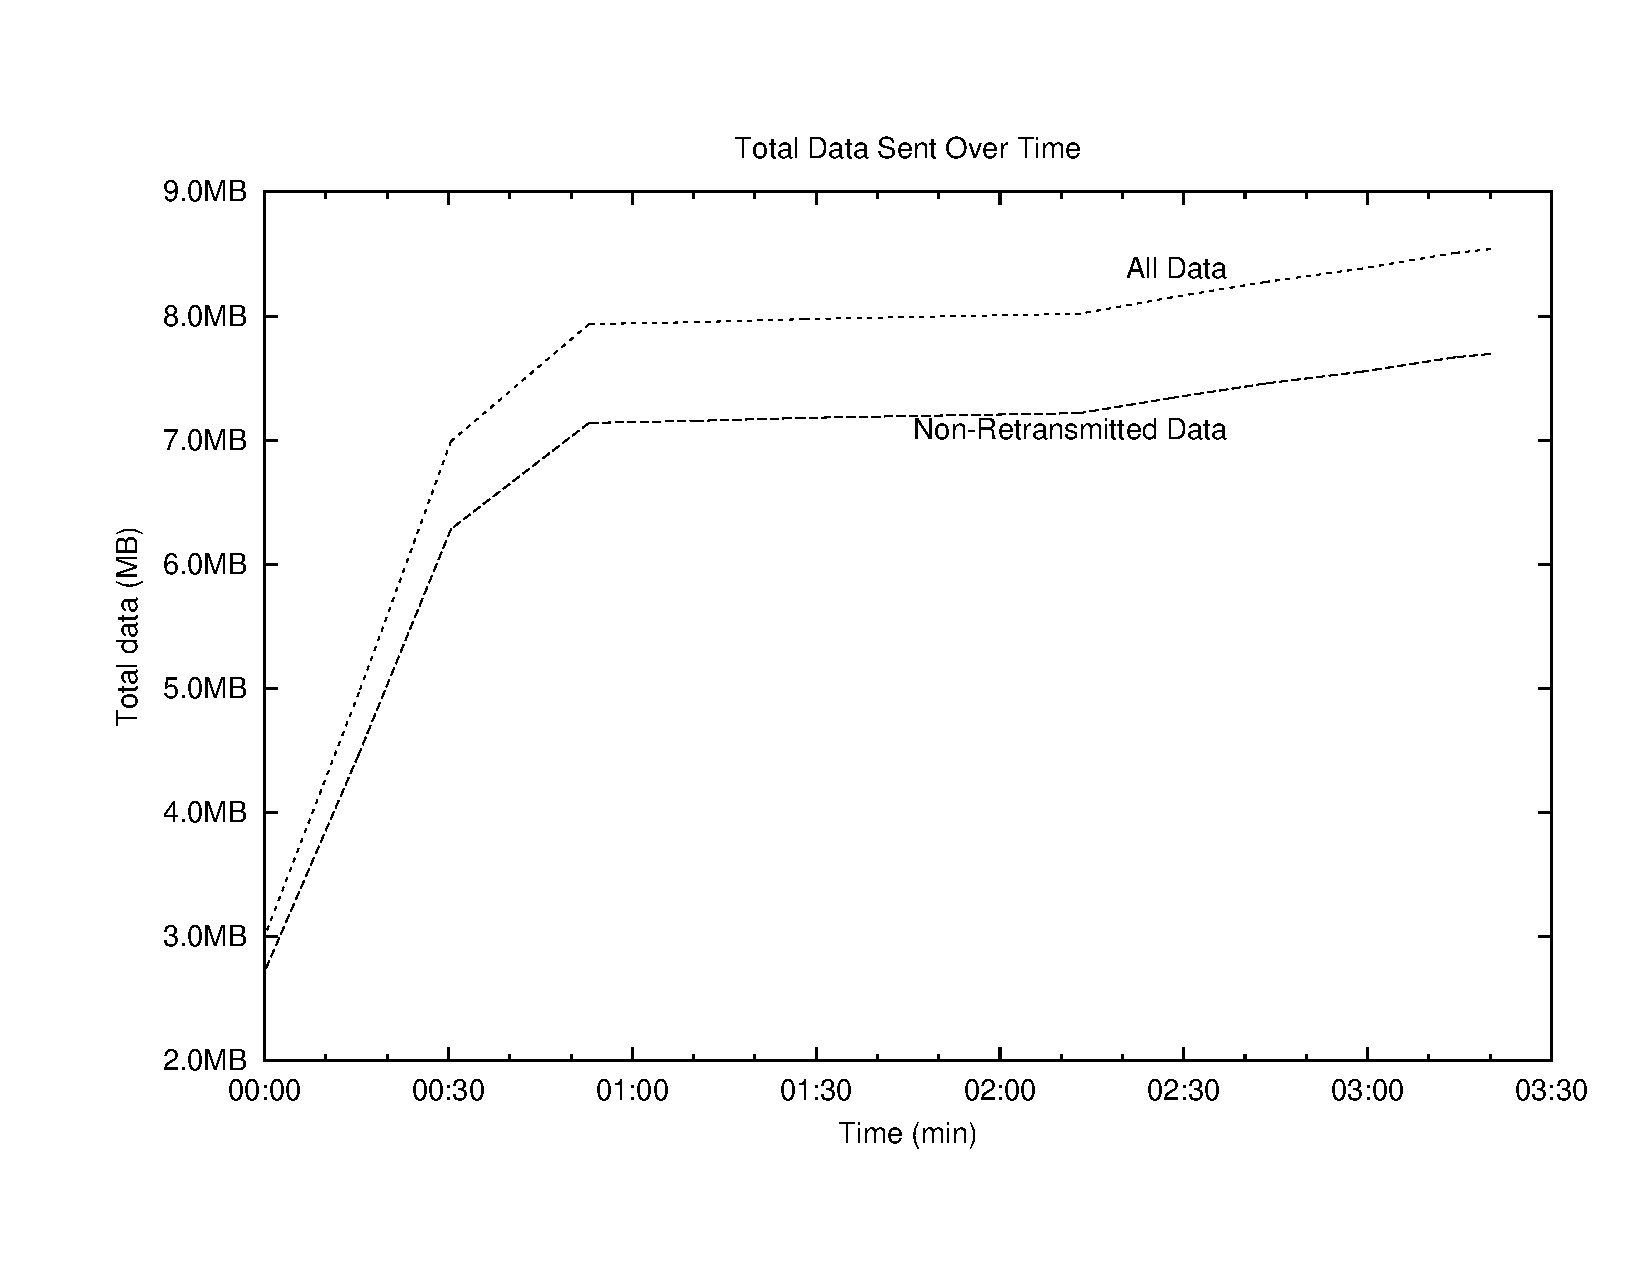
\includegraphics[height=10cm]{charts/dlna_traffic_10loss_data}
\caption{DLNA bad network traffic data chart \label{chart6}}
\end{figure}


\begin{figure}[htb]
\centering \includegraphics[height=10cm]{charts/AirPlay_traffic_15loss_data}
\caption{AirPlay bad network traffic data chart \label{chart6}}
\end{figure}
\begin{figure}[htb]
\centering 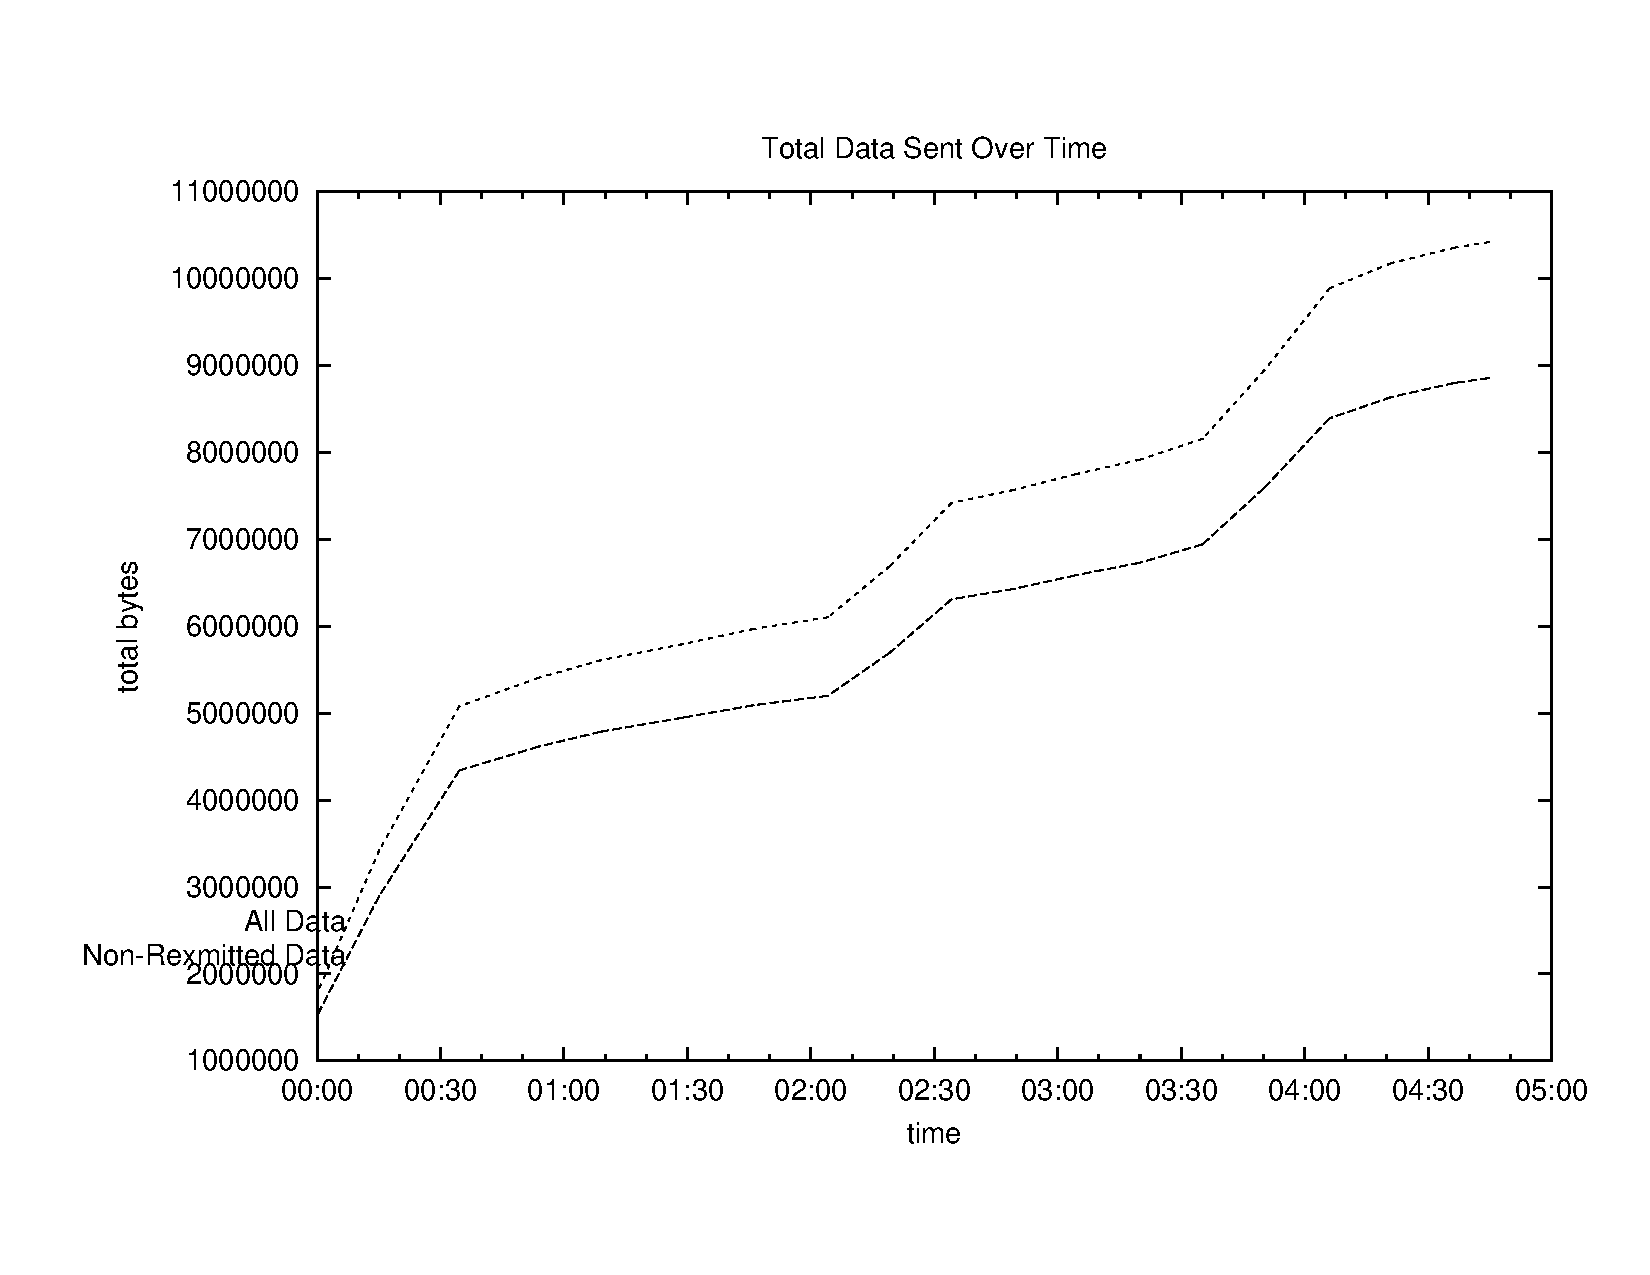
\includegraphics[height=10cm]{charts/dlna_traffic_15loss_data}
\caption{DLNA bad network traffic data chart \label{chart6}}
\end{figure}

\subsection{Statistics}
Through one year's on-line marketing, we reached 637000 downloads from 223
countries all around the world, with around 8000 daily active users. So far, the
average rating of our app is 3.9 out of 7527 ratings. The application turns out
to be popular in countries like France, United States, Germany, United Kingdom
and Brazil.

\begin{itemize}
\item[--]Totally more than 290000 downloads
\item[--]Used by people from 201 countries
\item[--]8000+ daily active users
\item[--]1,241,074 visits to home page
\item[--]Average rating 3.9, 3521 user gave rates
\item[--]On-line for 3 months
\end{itemize}
\begin{figure}[htb]
\centering 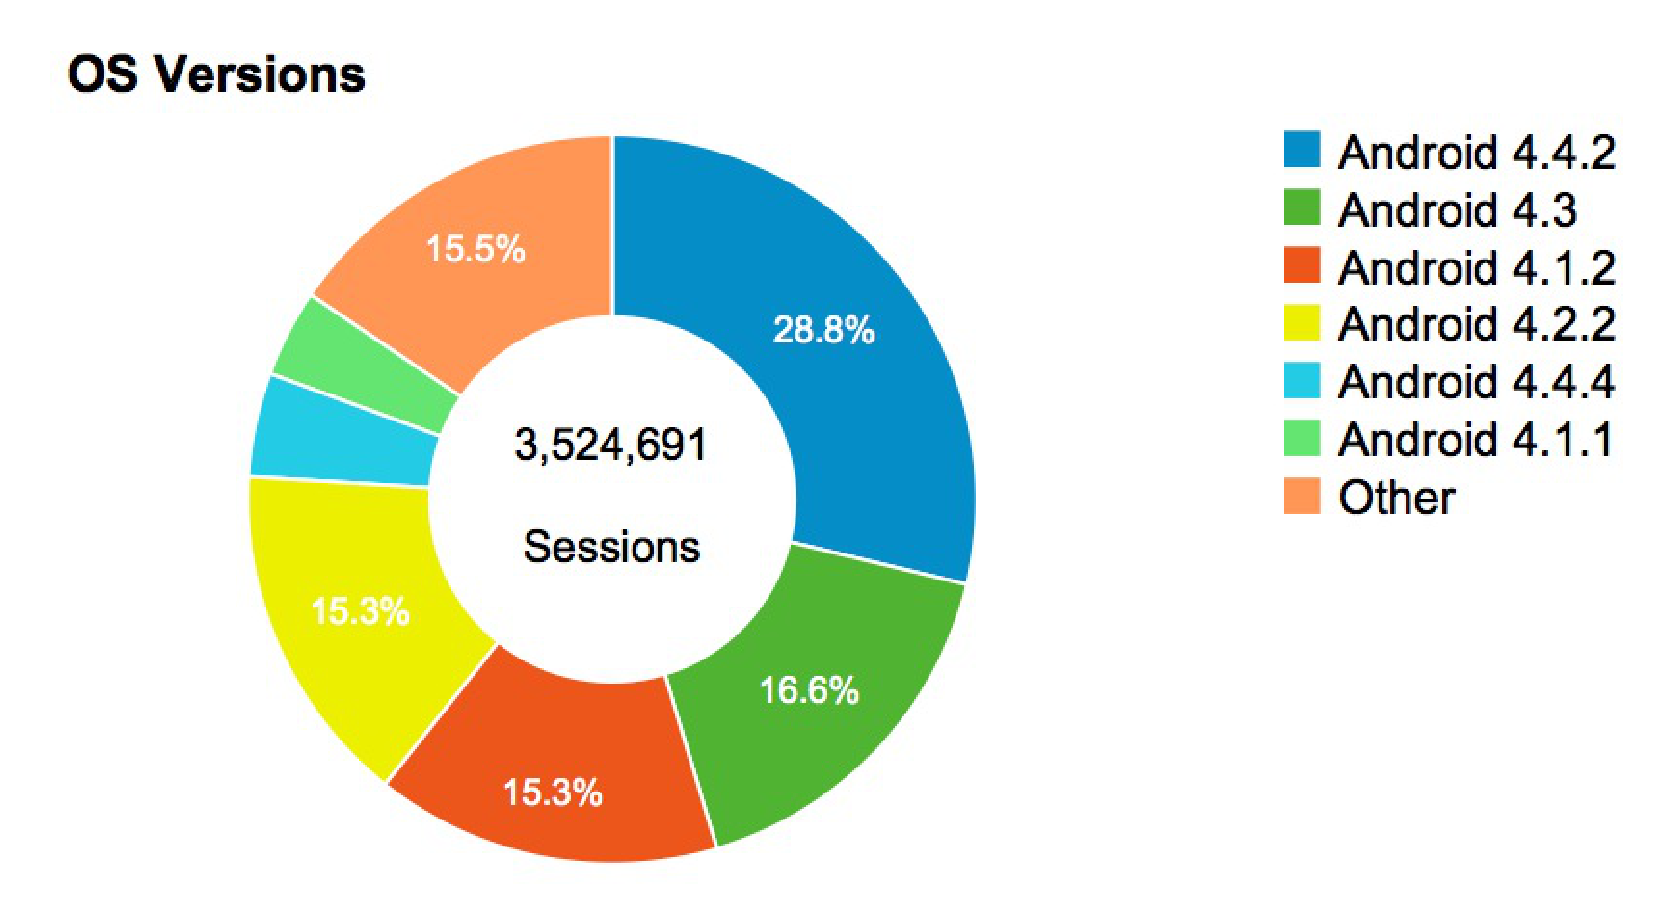
\includegraphics[height=5cm]{charts/android_versions}
\caption{Android versions \label{chart6}}
\end{figure}

\begin{figure}[htb]
\centering \includegraphics[height=9cm]{charts/user_world_map}
\caption{User world map \label{chart7}}
\end{figure}

\begin{table}[htb]
\caption{Receiver type statistic \label{Table8}}
\begin{center}
\fbox{
\begin{tabular}{c|l|l}  
\textbf{Device type } & Total selection & Percentage \\
\hline \textbf{AirPlay device} & 637446 & 39.72\\ \hline
\textbf{DLNA device} & 460139 & 28.67\\ \hline
\textbf{Phone speaker} & 353474 & 22.03\\ \hline
\textbf{Chromecast device} & 147333 & 9.18\\ \hline
\textbf{FireTV device} & 6368 & 0.40
\end{tabular}
}
\end{center}
\end{table}

\subsection{User study}
\begin{itemize}
\item[--]What information we can get back from users
\item[--]User behavior/ statistics
\item[--]Improve the application accordingly
\item[--]Strategies for decision making
\end{itemize}
Write result here.